% =============================================================================
% Section 2.2: Market Survey
% =============================================================================

\section{Market Survey}
\label{sec:market-survey}

This section surveys five representative platforms spanning corporate marketplace models, creator SaaS tools, open-source LMS software, institutional partnerships, and WordPress plugin ecosystems. Each subsection follows a consistent analytical frame: platform description, publicly known technical architecture, strengths (\textit{pros}), weaknesses relative to NexaLearn (\textit{cons}), and strategic implications for positioning. The survey is based on publicly available documentation, vendor pricing pages, and industry analyses current to the 2025--2026 academic reporting period; proprietary internal architectures of closed platforms are inferred from observable API surfaces and engineering blog posts where available.

A consolidated comparison appears in Table~\ref{tab:platform-comparison} following the competitor subsections.

\subsection{Udemy for Business and Udemy-Like Marketplace Platforms}
\label{subsec:udemy}

\textbf{Description.}
Udemy is the world's largest consumer marketplace for online courses, hosting more than 200,000 courses and tens of millions of learners. \textbf{Udemy for Business (UFB)} is the enterprise-facing product offering curated course libraries, analytics dashboards, and LMS integrations for corporate training teams. Similar marketplace-centric platforms include LinkedIn Learning and Pluralsight, which combine proprietary content libraries with subscription access models rather than enabling organisations to operate fully custom backends.

\textbf{Technical architecture (public knowledge).}
Udemy operates a proprietary microservices architecture deployed on cloud infrastructure, with internal services for content delivery, recommendation, payment settlement, and anti-piracy DRM not exposed to customers. Public APIs for UFB focus on user provisioning (SCIM), progress reporting (xAPI subsets), and catalogue embedding---not on course authoring, payment routing, or video pipeline customisation. Video delivery relies on proprietary CDN and transcoding stacks optimised for global scale rather than customer-configurable providers such as Mux.

\textbf{Pros.}
\begin{itemize}
  \item \textbf{Massive scale and reliability} --- battle-tested infrastructure serving millions of concurrent learners worldwide;
  \item \textbf{Content marketplace} --- immediate access to thousands of professional courses without content creation overhead;
  \item \textbf{Brand recognition} --- reduces procurement friction for corporate L\&D buyers familiar with the consumer product;
  \item \textbf{Analytics maturity} --- established completion and skills reporting for enterprise HR integrations.
\end{itemize}

\textbf{Cons.}
\begin{itemize}
  \item \textbf{Closed-source and non-customisable backend} --- no access to enrollment logic, event pipelines, or assessment engines;
  \item \textbf{Revenue-sharing and licensing costs} --- creators on consumer Udemy receive 37--97\% revenue share depending on acquisition channel; UFB involves per-seat enterprise licensing beyond customer control;
  \item \textbf{No DDD/Clean Architecture reference} --- zero educational value for engineering teams studying modern backend patterns;
  \item \textbf{Limited AI quiz generation} --- AI features (if present) are platform-controlled black boxes, not extensible Whisper/LLM pipelines;
  \item \textbf{Vendor lock-in} --- migration of course data, progress records, and payment history off-platform is intentionally difficult;
  \item \textbf{No self-hosting} --- incompatible with university data-sovereignty requirements addressed by NexaLearn.
\end{itemize}

\subsection{Teachable and Thinkific}
\label{subsec:teachable-thinkific}

\textbf{Description.}
\textbf{Teachable} and \textbf{Thinkific} are leading SaaS platforms targeting independent course creators, coaches, and small academies. They provide drag-and-drop course builders, landing pages, email marketing integrations, affiliate programmes, and built-in checkout experiences. Both platforms prioritise time-to-first-sale over backend extensibility, positioning themselves as ``business-in-a-box'' solutions for non-technical creators.

\textbf{Technical architecture (public knowledge).}
Both platforms operate multi-tenant closed backends (likely Ruby on Rails or similar monolithic/SaaS stacks internally, though not publicly confirmed). Creators interact primarily through web dashboards; limited public REST APIs support enrolment webhooks, coupon management, and third-party automation via Zapier. Video hosting is bundled---Teachable migrated to native video hosting; Thinkific offers built-in hosting with CDN delivery. Payment processing integrates Stripe and PayPal on behalf of creators, with platforms acting as merchant-of-record or payment facilitator depending on plan tier.

\textbf{Pros.}
\begin{itemize}
  \item \textbf{Rapid creator onboarding} --- first course publishable within hours without engineering staff;
  \item \textbf{Integrated marketing tooling} --- sales pages, coupons, and affiliate tracking reduce need for external tools;
  \item \textbf{Stripe integration out-of-the-box} --- creators receive payment processing without PCI compliance burden;
  \item \textbf{Established user bases} --- large creator communities, template libraries, and support documentation;
  \item \textbf{Predictable SaaS pricing} --- subscription tiers (\$39--\$499/month) versus custom development costs.
\end{itemize}

\textbf{Cons.}
\begin{itemize}
  \item \textbf{Closed-source with restricted API access} --- cannot modify enrollment state machines, outbox patterns, or assessment algorithms;
  \item \textbf{Platform transaction fees} --- Teachable charges 5\% transaction fees on Basic plans plus payment processing; Thinkific charges 0--5\% depending on tier;
  \item \textbf{No AI-native quiz generation pipeline} --- assessments are manually authored; no Whisper/LLM integration comparable to NexaLearn's AI Pipeline context;
  \item \textbf{Video processing opacity} --- creators cannot swap Mux for alternative encoders or implement custom DRM policies;
  \item \textbf{No DDD architecture} --- unsuitable as an engineering reference for Computer Engineering curricula;
  \item \textbf{Vendor lock-in} --- course content, student lists, and payment history export with incomplete API coverage;
  \item \textbf{Limited white-label depth} --- custom domains available but backend remains platform-controlled multi-tenant infrastructure.
\end{itemize}

\subsection{Moodle (Open-Source LMS)}
\label{subsec:moodle}

\textbf{Description.}
\textbf{Moodle} is the dominant open-source Learning Management System globally, powering institutions from primary schools to research universities. It provides course management, forums, quizzes, gradebooks, SCORM players, and thousands of community plugins. Moodle's GPL licence and self-hosting support have made it the default choice for budget-conscious institutions worldwide.

\textbf{Technical architecture (public knowledge).}
Moodle is a PHP monolith using a plugin architecture layered atop a relational database (typically MySQL/MariaDB or PostgreSQL). Core subsystems include mod (activity modules), auth plugins, enrol plugins, and theme engines. Background tasks run via cron; caching supports Redis/Memcached. Version 4.x introduces modernised UI (Boost theme) but retains the fundamental plugin-sprawl architecture. There is no native event-driven outbox, bounded context separation, or TypeScript type safety across module boundaries.

\textbf{Pros.}
\begin{itemize}
  \item \textbf{Open source and self-hostable} --- full source access, no per-seat licensing, data sovereignty;
  \item \textbf{Massive installed base} --- extensive community, plugin ecosystem, and institutional familiarity;
  \item \textbf{Feature breadth} --- gradebooks, workshops, Wikis, SCORM, competencies, and proctoring plugins;
  \item \textbf{Academic credibility} --- decades of pedagogical feature accumulation validated in accreditation contexts;
  \item \textbf{Global localisation} --- interface packs in 100+ languages.
\end{itemize}

\textbf{Cons.}
\begin{itemize}
  \item \textbf{Legacy monolithic architecture} --- plugin interdependencies create maintenance burden; no DDD or Clean Architecture guidance;
  \item \textbf{PHP stack divergence} --- modern edtech startups prefer TypeScript/Node.js talent pools over PHP plugin development;
  \item \textbf{No native Stripe/Mux/AI pipeline integration} --- requires custom plugins of varying quality; payment and video remain fragmented;
  \item \textbf{AI features via third-party plugins only} --- no unified Whisper/LLM quiz generation context; inconsistent security models across plugins;
  \item \textbf{Operational complexity at scale} --- large deployments require careful cron tuning, caching layers, and database optimisation without cloud-native defaults comparable to Docker Compose NestJS stacks;
  \item \textbf{Developer experience} --- lacks OpenAPI-first REST design, Prisma-type safety, and Testcontainers integration testing patterns exemplified by NexaLearn.
\end{itemize}

\subsection{Coursera for Campus}
\label{subsec:coursera}

\textbf{Description.}
\textbf{Coursera for Campus} (and related Coursera for Business products) provides universities and enterprises access to Coursera's catalogue of courses and degrees, combined with tools for instructors to author private courses, manage programmes, and track learner progress. Coursera partners with top global universities for branded content, positioning the platform as a premium institutional channel rather than a self-hosted backend framework.

\textbf{Technical architecture (public knowledge).}
Coursera operates a proprietary cloud-native platform originally built on Scala/Play Framework microservices (per early engineering publications), with specialised services for video streaming, peer grading, item response theory assessments, and identity verification. Integrations include LTI for LMS embedding, API access for enterprise reporting, and SSO via SAML. The platform is entirely SaaS-hosted on Coursera infrastructure; institutions do not receive backend source code or database access.

\textbf{Pros.}
\begin{itemize}
  \item \textbf{Premium content library} --- immediate access to courses from Stanford, Google, IBM, and partner universities;
  \item \textbf{Institutional brand association} --- credibility for universities offering co-branded programmes;
  \item \textbf{Scalable video and assessment infrastructure} --- handles massive concurrent MOOC enrolments;
  \item \textbf{Guided projects and hands-on labs} --- mature interactive content formats;
  \item \textbf{Some AI integration} --- Coursera Coach and AI-assisted learning features emerging in 2024--2025 product releases.
\end{itemize}

\textbf{Cons.}
\begin{itemize}
  \item \textbf{Fully closed-source} --- zero backend customisation; institutions are tenants, not owners;
  \item \textbf{High institutional licensing costs} --- per-student or per-programme fees scale expensively compared to self-hosted NexaLearn;
  \item \textbf{No DDD reference or API completeness} --- integration limited to prescribed LTI and reporting endpoints;
  \item \textbf{AI features not extensible} --- institutions cannot deploy custom Whisper/LLM pipelines or modify quiz generation logic;
  \item \textbf{Payment integration opaque} --- Coursera manages monetisation for partner content; private course payment flows constrained;
  \item \textbf{Vendor lock-in and data portability limits} --- migrating authored content and learner records off-platform is restricted;
  \item \textbf{Limited relevance for custom edtech startups} --- business model assumes catalogue leverage, not greenfield platform construction.
\end{itemize}

\subsection{LearnDash (WordPress LMS Plugin)}
\label{subsec:learndash}

\textbf{Description.}
\textbf{LearnDash} is a commercial WordPress plugin transforming a standard WordPress site into an LMS with courses, lessons, topics, quizzes, certificates, and drip-feed content scheduling. It targets creators and small businesses already invested in the WordPress ecosystem, leveraging familiar admin UI and the vast WordPress plugin marketplace for commerce (WooCommerce), membership (MemberPress), and page building (Elementor).

\textbf{Technical architecture (public knowledge).}
LearnDash extends WordPress's PHP/MySQL architecture with custom post types for courses and lessons, WordPress hooks for lifecycle events, and Gutenberg blocks for frontend rendering. Quizzes use proprietary question engines; video lessons embed via shortcodes supporting YouTube, Vimeo, or self-hosted MP4. Payments integrate through WooCommerce or native Stripe/PayPal add-ons. The architecture inherits WordPress's request-per-page model, transients API for caching, and wp-cron for scheduled tasks---fundamentally different from NestJS microservice-ready modular monoliths.

\textbf{Pros.}
\begin{itemize}
  \item \textbf{Low entry cost for WordPress users} --- leverages existing hosting, themes, and SEO workflows;
  \item \textbf{GPL-licensed core plugin} --- source readable; large WordPress developer community for extensions;
  \item \textbf{Integrated commerce via WooCommerce} --- mature payment plugin ecosystem;
  \item \textbf{Certificate and drip content features} --- adequate for solo creators and small academies;
  \item \textbf{Affordable licensing} --- approximately \$199/year for single-site plugin licence versus enterprise LMS contracts.
\end{itemize}

\textbf{Cons.}
\begin{itemize}
  \item \textbf{WordPress architectural constraints} --- not designed for high-concurrency API-first backends; scaling requires caching plugins and database tuning rather than horizontal stateless API tiers;
  \item \textbf{No DDD, outbox, or event-driven reliability patterns} --- enrollment/payment race conditions handled ad hoc via WordPress post meta;
  \item \textbf{Video processing limited} --- no Mux-grade transcoding pipeline; relies on external hosts or raw MP4 uploads without adaptive bitrate streaming defaults;
  \item \textbf{AI quiz generation absent natively} --- requires separate WordPress AI plugins with inconsistent quality and security;
  \item \textbf{Security surface area} --- WordPress's plugin ecosystem is a frequent attack target; institutional IT departments often resist WordPress for regulated training data;
  \item \textbf{Not a developer reference architecture} --- unsuitable for Computer Engineering graduation projects demonstrating NestJS, Prisma, and transactional outbox patterns;
  \item \textbf{Vendor dependency on LearnDash updates} --- major WordPress or LearnDash version incompatibilities can break production sites.
\end{itemize}

\subsection{Competitive Comparison Summary}
\label{subsec:comparison-summary}

Table~\ref{tab:platform-comparison} consolidates the market survey into a single reference matrix. NexaLearn is included as the proposed alternative to highlight differentiated capabilities. Rating conventions: \textbf{Yes} = first-class native support; \textbf{Partial} = available via plugins, limited APIs, or opaque platform features; \textbf{No} = not meaningfully supported; \textbf{N/A} = not applicable to platform business model.

\begin{table}[H]
  \centering
  \caption{Competitive Platform Comparison (Table 2.1)}
  \label{tab:platform-comparison}
  \footnotesize
  \setlength{\tabcolsep}{3pt}
  \begin{tabular}{@{}p{2.1cm} c c c c c p{2.4cm}@{}}
    \toprule
    \textbf{Platform} &
    \textbf{Open Source} &
    \textbf{AI Features} &
    \textbf{Video Processing} &
    \textbf{Payment Integration} &
    \textbf{DDD Architecture} &
    \textbf{Price (indicative)} \\
    \midrule
    Udemy / UFB &
    No &
    Partial &
    Proprietary CDN &
    Proprietary &
    No &
    Per-seat enterprise; creator revenue share \\
    \addlinespace
    Teachable &
    No &
    No &
    Built-in hosting &
    Stripe (built-in) &
    No &
    \$39--\$499/mo + transaction fees \\
    \addlinespace
    Thinkific &
    No &
    No &
    Built-in hosting &
    Stripe/PayPal &
    No &
    \$0--\$499/mo + transaction fees \\
    \addlinespace
    Moodle &
    Yes &
    Partial (plugins) &
    Plugin-dependent &
    Plugin-dependent &
    No &
    Free (GPL) + hosting/support costs \\
    \addlinespace
    Coursera Campus &
    No &
    Partial (platform AI) &
    Proprietary &
    Proprietary &
    No &
    Institutional licence (per student) \\
    \addlinespace
    LearnDash &
    Partial (GPL plugin) &
    No (plugins only) &
    Basic embed/host &
    WooCommerce/Stripe &
    No &
    \~\$199/yr plugin + WordPress hosting \\
    \addlinespace
    \textbf{NexaLearn (proposed)} &
    \textbf{Yes} &
    \textbf{Yes (Whisper/LLM)} &
    \textbf{Mux integration} &
    \textbf{Stripe (native)} &
    \textbf{Yes} &
    \textbf{OSS core + \$5,000/yr enterprise support} \\
    \bottomrule
  \end{tabular}
\end{table}

\begin{figure}[H]
  \centering
  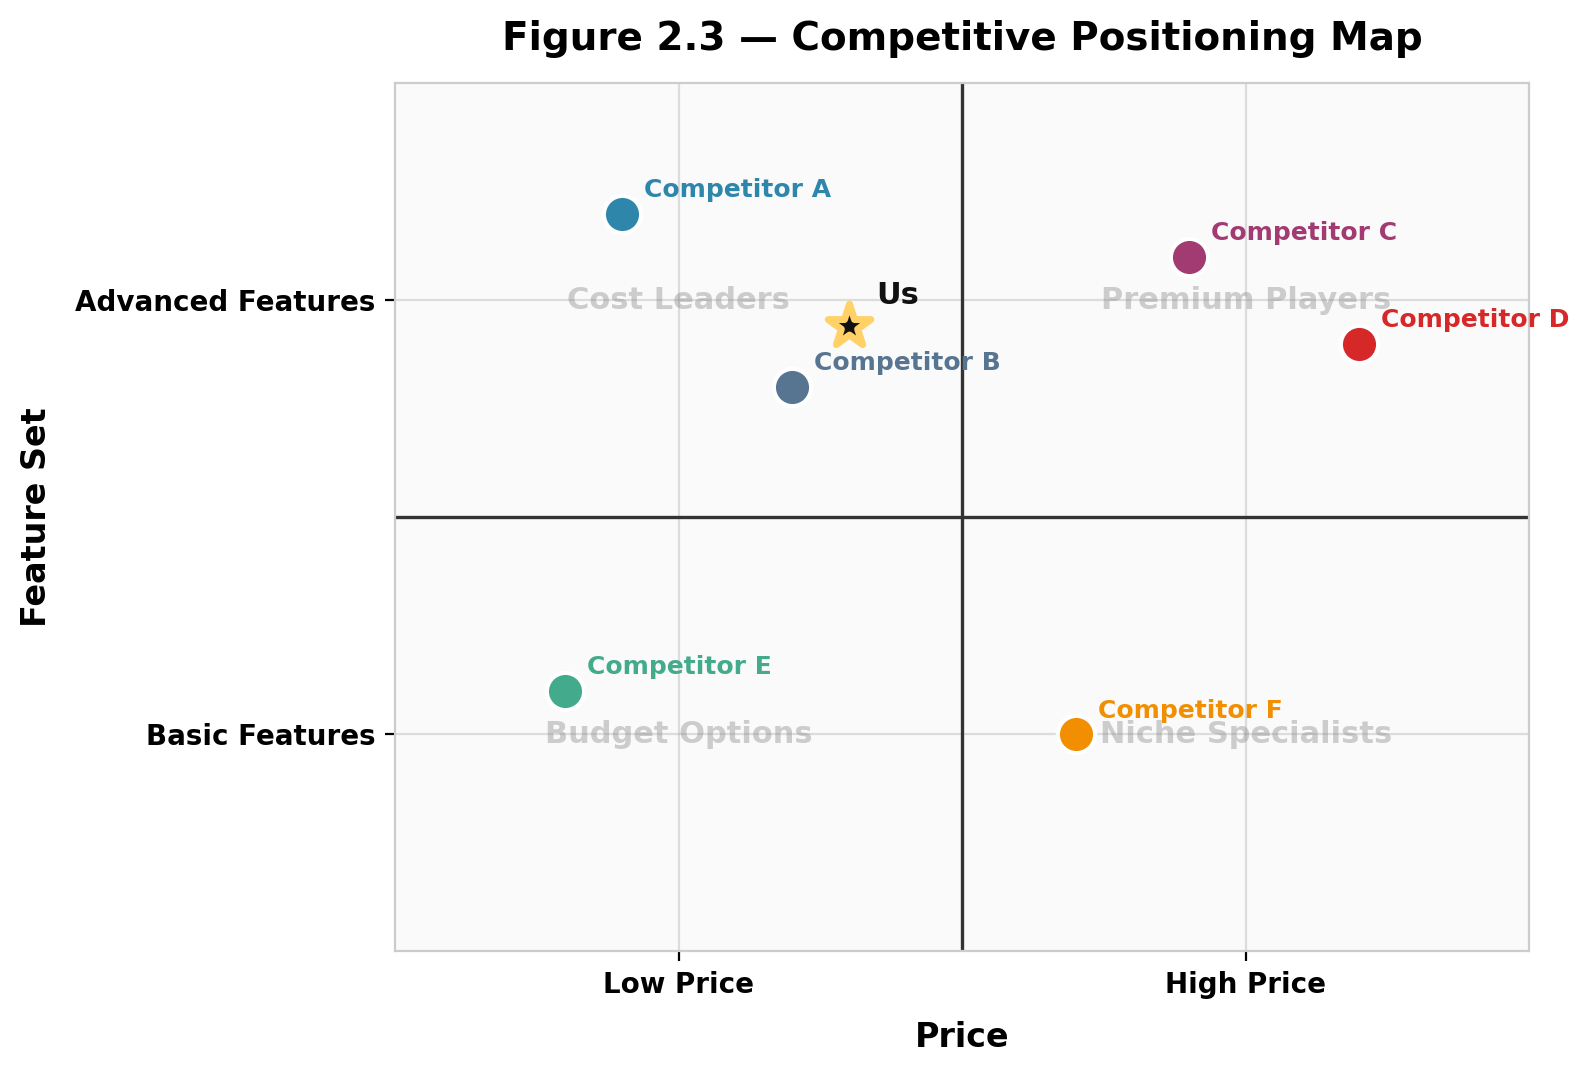
\includegraphics[width=0.90\textwidth]{images/competitive_positioning.png}
  \caption{Competitive Positioning: Architectural Openness versus Backend Customisation Depth}
  \label{fig:competitive-positioning}
\end{figure}

Figure~\ref{fig:competitive-positioning} visualises the strategic whitespace NexaLearn occupies: higher architectural openness and DDD discipline than closed SaaS platforms, and more modern API-first engineering than legacy Moodle/WordPress stacks. No surveyed competitor simultaneously offers open source, native Stripe/Mux/AI pipeline integration, and an explicit DDD modular monolith reference---validating the market gap identified in Chapter~\ref{ch:introduction}.

In conclusion, the market survey demonstrates that while each competing platform excels within its niche---Udemy's catalogue scale, Teachable's creator UX, Moodle's institutional adoption, Coursera's academic partnerships, LearnDash's WordPress accessibility---none delivers NexaLearn's combination of \textit{open-source extensibility}, \textit{production reliability patterns}, and \textit{AI-augmented backend completeness}. The following section translates this positioning into a quantified business case and financial analysis.
